\let\negmedspace\undefined
\let\negthickspace\undefined
\documentclass[journal,12pt,onecolumn]{IEEEtran}
\usepackage{cite}
\usepackage{amsmath,amssymb,amsfonts,amsthm}
\usepackage{algorithmic}
\usepackage{graphicx}
\usepackage{textcomp}
\usepackage{xcolor}
\usepackage{txfonts}
\usepackage{listings}
\usepackage{enumitem}
\usepackage{mathtools}
\usepackage{gensymb}
\usepackage[breaklinks=true]{hyperref}
\usepackage{tkz-euclide} % loads  TikZ and tkz-base
\usepackage{listings}



\newtheorem{theorem}{Theorem}[section]
\newtheorem{problem}{Problem}
\newtheorem{proposition}{Proposition}[section]
\newtheorem{lemma}{Lemma}[section]
\newtheorem{corollary}[theorem]{Corollary}
\newtheorem{example}{Example}[section]
\newtheorem{definition}[problem]{Definition}
%\newtheorem{thm}{Theorem}[section] 
%\newtheorem{defn}[thm]{Definition}
%\newtheorem{algorithm}{Algorithm}[section]
%\newtheorem{cor}{Corollary}
\newcommand{\BEQA}{\begin{eqnarray}}
\newcommand{\EEQA}{\end{eqnarray}}
\newcommand{\system}[1]{\stackrel{#1}{\rightarrow}}
\newcommand{\define}{\stackrel{\triangle}{=}}
\theoremstyle{remark}
\newtheorem{rem}{Remark}
%\bibliographystyle{ieeetr}
\begin{document}
%
\providecommand{\pr}[1]{\ensuremath{\Pr\left(#1\right)}}
\providecommand{\prt}[2]{\ensuremath{p_{#1}^{\left(#2\right)} }}        % own macro for this question
\providecommand{\qfunc}[1]{\ensuremath{Q\left(#1\right)}}
\providecommand{\sbrak}[1]{\ensuremath{{}\left[#1\right]}}
\providecommand{\lsbrak}[1]{\ensuremath{{}\left[#1\right.}}
\providecommand{\rsbrak}[1]{\ensuremath{{}\left.#1\right]}}
\providecommand{\brak}[1]{\ensuremath{\left(#1\right)}}
\providecommand{\lbrak}[1]{\ensuremath{\left(#1\right.}}
\providecommand{\rbrak}[1]{\ensuremath{\left.#1\right)}}
\providecommand{\cbrak}[1]{\ensuremath{\left\{#1\right\}}}
\providecommand{\lcbrak}[1]{\ensuremath{\left\{#1\right.}}
\providecommand{\rcbrak}[1]{\ensuremath{\left.#1\right\}}}
\newcommand{\sgn}{\mathop{\mathrm{sgn}}}
\providecommand{\abs}[1]{\left\vert#1\right\vert}
\providecommand{\res}[1]{\Res\displaylimits_{#1}} 
\providecommand{\norm}[1]{\left\lVert#1\right\rVert}
%\providecommand{\norm}[1]{\lVert#1\rVert}
\providecommand{\mtx}[1]{\mathbf{#1}}
\providecommand{\mean}[1]{E\left[ #1 \right]}
\providecommand{\cond}[2]{#1\middle|#2}
\providecommand{\fourier}{\overset{\mathcal{F}}{ \rightleftharpoons}}
\newenvironment{amatrix}[1]{%
  \left(\begin{array}{@{}*{#1}{c}|c@{}}
}{%
  \end{array}\right)
}
%\providecommand{\hilbert}{\overset{\mathcal{H}}{ \rightleftharpoons}}
%\providecommand{\system}{\overset{\mathcal{H}}{ \longleftrightarrow}}
	%\newcommand{\solution}[2]{\textbf{Solution:}{#1}}
\newcommand{\solution}{\noindent \textbf{Solution: }}
\newcommand{\cosec}{\,\text{cosec}\,}
\providecommand{\dec}[2]{\ensuremath{\overset{#1}{\underset{#2}{\gtrless}}}}
\newcommand{\myvec}[1]{\ensuremath{\begin{pmatrix}#1\end{pmatrix}}}
\newcommand{\mydet}[1]{\ensuremath{\begin{vmatrix}#1\end{vmatrix}}}
\newcommand{\myaugvec}[2]{\ensuremath{\begin{amatrix}{#1}#2\end{amatrix}}}
\providecommand{\rank}{\text{rank}}
\providecommand{\pr}[1]{\ensuremath{\Pr\left(#1\right)}}
\providecommand{\qfunc}[1]{\ensuremath{Q\left(#1\right)}}
	\newcommand*{\permcomb}[4][0mu]{{{}^{#3}\mkern#1#2_{#4}}}
\newcommand*{\perm}[1][-3mu]{\permcomb[#1]{P}}
\newcommand*{\comb}[1][-1mu]{\permcomb[#1]{C}}
\providecommand{\qfunc}[1]{\ensuremath{Q\left(#1\right)}}
\providecommand{\gauss}[2]{\mathcal{N}\ensuremath{\left(#1,#2\right)}}
\providecommand{\diff}[2]{\ensuremath{\frac{d{#1}}{d{#2}}}}
\providecommand{\myceil}[1]{\left \lceil #1 \right \rceil }
\newcommand\figref{Fig.~\ref}
\newcommand\tabref{Table~\ref}
\newcommand{\sinc}{\,\text{sinc}\,}
\newcommand{\rect}{\,\text{rect}\,}
%%
%	%\newcommand{\solution}[2]{\textbf{Solution:}{#1}}
%\newcommand{\solution}{\noindent \textbf{Solution: }}
%\newcommand{\cosec}{\,\text{cosec}\,}
%\numberwithin{equation}{section}
%\numberwithin{equation}{subsection}
%\numberwithin{problem}{section}
%\numberwithin{definition}{section}
%\makeatletter
%\@addtoreset{figure}{problem}
%\makeatother

%\let\StandardTheFigure\thefigure
\let\vec\mathbf


\bibliographystyle{IEEEtran}
\title{SEQUENCE AND SERIES}
\author{EE23BTECH11059- Tejas Mehtre$^{*}$% <-this % stops a space
}
\maketitle




\bigskip

\renewcommand{\thefigure}{\theenumi}
\renewcommand{\thetable}{\theenumi}
%\renewcommand{\theequation}{\theenumi}
Find the sum of first 51 terms of an AP whose second and third terms are 14 and 18 respectively. \\
    \solution
    \begin{table}[!ht]
    \centering
        \begin{tabular}{|c|c|c|} 
      \hline
\textbf{Variable}& \textbf{Description}& \textbf{Value}\\\hline
        $x(1)$& Second term of $AP$ & $14$ \\ \hline
        $x(2)$ &Third term of $AP$ & $18$ \\ \hline
         $x(0)$ & First term of $AP$ & $2x(1)-x(2)=10$ \\ \hline
         $d$ & Common difference of $AP$ $(x(2)-x(1))$ & $4$ \\ \hline
          $x(n)$& $n^{th}$ term of sequence& $(4n+10)u(n)$\\ \hline 
          
    \end{tabular}

    \caption{input parameters}
    \label{}
\end{table}
    
       For an $AP$,
\begin{align}
    X\brak z &= \frac{ x\brak 0 }{1-z^{-1}} + \frac{dz^{-1}}{{(1-z^{-1})}^{2}}    \\
    \implies X\brak z &= \frac{10}{(1-z^{-1})} + \frac{4z^{-1}}{{(1-z^{-1})}^{2}}, \abs{z}>1    \\
    y\brak{n}&=x\brak{n}\ast u\brak{n}\\
     Y\brak{z}&=X\brak{z}U\brak{z}   \\
     Y\brak z &= \frac{10}{(1-z^{-1})^{2}} + \frac{4z^{-1}}{{(1-z^{-1})}^{3}} \\  
     \implies Y\brak z &= \frac{(-6z^{-1}+10)}{(1-z^{-1})^{3}} , \abs{z}>1
\end{align}
Using Contour Integration to find the inverse $Z$-transform,
\begin{align}
    y(50)&=\frac{1}{2\pi j}\oint_{C}Y(z) \;z^{49} \;dz  \\
    &=\frac{1}{2\pi j}\oint_{C}\frac{(-6z^{-1}+10)z^{49}}{({1-z^{-1})}^{3}} \;dz 
\end{align}
We can observe that the pole is repeated $3$ times and thus $m=3$,
\begin{align}
    R&=\frac{1}{\brak {m-1}!}\lim\limits_{z\to a}\frac{d^{m-1}}{dz^{m-1}}\brak {{(z-a)}^{m}f\brak z}  \\
    \implies R &=\frac{1}{\brak {2}!}\lim\limits_{z\to 1}\frac{d^{2}}{dz^{2}}\brak {{(z-1)}^{3}\frac{(-6z^{-1}+10)z^{52}}{{(z-1)}^3}}   \\
    \implies R &=\frac{1}{2}\lim\limits_{z\to 1}\frac{d^2}{dz^2}(10z^{52}-6z^{51})   \\
    \implies R &=5610 \\
    \therefore y(50)&=5610
\end{align}

\begin{figure}[ht]
        \centering
        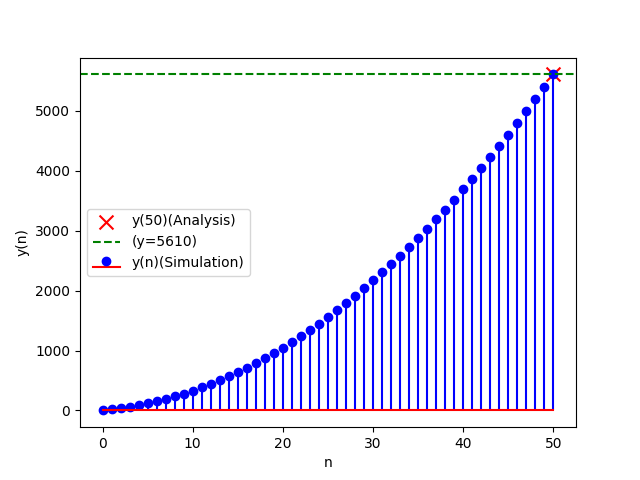
\includegraphics[width=\columnwidth]{figs/plot.png}
        \caption{Plot of x(n) $vs$ n}
    \end{figure}
    
\begin{figure}[ht]
        \centering
        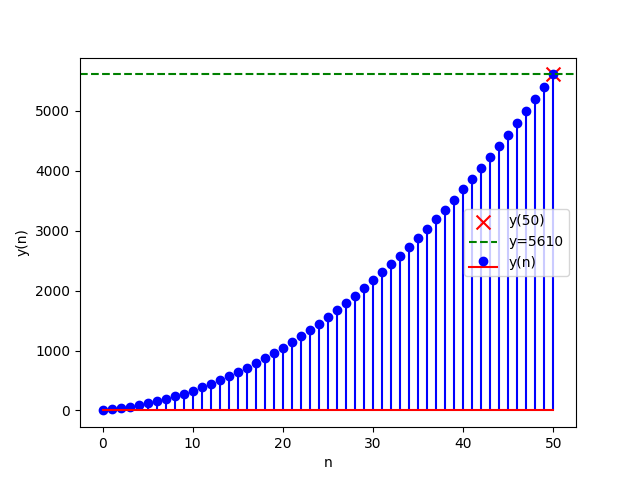
\includegraphics[width=\columnwidth]{figs/plot2.png}
        \caption{Analysis vs Simulation}
    \end{figure}
\end{document}
